%----------------------------------------------------------------------------------------
%	HOMEWORK ASSIGNMENT CSCI 5525
%----------------------------------------------------------------------------------------

%----------------------------------------------------------------------------------------
%	PROLOUGE 
%----------------------------------------------------------------------------------------
\documentclass[a4paper, 11pt]{article}
\usepackage[scale=0.85]{geometry} 		% Reduce document margins
\usepackage{hyperref} 					% Required for hyperlinks i.e. e-mail %
\usepackage{titlesec} 					% Used to customize the \section command
\usepackage[T1]{fontenc}				% Used to have both Bold and Small caps in heading
\usepackage{amsmath}					% Used to write equations
\usepackage{amssymb}					% Used to write math symbols e.g. R = real number set
\usepackage{autobreak}
\usepackage{graphicx}					% Used to include images
\usepackage{tabularx} 					% For custom table %
\usepackage{mathtools}
\usepackage{subfig}
\usepackage{bbm}						% For vector 1
%----------------------------------------------------------------------------------------
%	CUSTOM MACRO DEFINITION AND ENVIRONMENT MODIFICATION
%----------------------------------------------------------------------------------------
\titleformat{\section}{\bfseries\Large\scshape\filcenter}{}{0em}{}[{\titlerule[1pt]}] % Text formatting of sections
\titlespacing{\section}{0pt}{3pt}{3pt} % Spacing around sections
\pagestyle{empty} % Removes page numbering
\newcommand{\xVec}{\ensuremath{\boldsymbol{x}}}
\newcommand{\wVec}{\ensuremath{\boldsymbol{w}}}
\newcommand{\muVec}{\ensuremath{\boldsymbol{\mu}}}
\newcommand{\mVec}{\ensuremath{\boldsymbol{m}}}
\newcommand{\sVec}{\ensuremath{\boldsymbol{S}}}
\newcommand{\sigmaVec}{\ensuremath{\boldsymbol{\sigma}}}
\newcommand{\SigmaVec}{\ensuremath{\boldsymbol{\Sigma}}}
\DeclareMathOperator*{\minimize}{minimize}
\DeclareMathOperator*{\argmax}{arg\,max}
\DeclareMathOperator*{\argmin}{arg\,min}
%----------------------------------------------------------------------------------------
%	MAIN BODY
%----------------------------------------------------------------------------------------
\begin{document}
	%----------------------------------------------------------------------------------------
%	HEADER
%----------------------------------------------------------------------------------------
\section{HW 4}
\begin{tabularx}{\textwidth}{l}
	\hspace*{-0.8cm}\large\textsc{Arnab Dey}\\
	\hspace*{-0.8cm}Student ID: 5563169\\
	\hspace*{-0.8cm}Email: dey00011@umn.edu\\
\end{tabularx}
\bigskip
\par
    %----------------------------------------------------------------------------------------
%	SOLUTION 1.a
%----------------------------------------------------------------------------------------
\subsection*{Solution 1.a}
Kernel function $K_i(x, x^{\prime})$ is defined as
\begin{align*}
	K_i(x, x^{\prime}) = \phi_i(x)^T\phi_i(x^{\prime}),
\end{align*}
where $x, x \in \mathbb{R}^p$, and  $\phi(x) \in \mathbb{R}^d$ is a feature space transformation. Note, that a valid kernel function is symmetric and positive semidefinite. Let $K_1, K_2, \ldots, K_m$ be a set of valid kernel functions. Therefore, for any $w_j \geq 0, j=1,2,\ldots,m$
\begin{align*}
	K(x, x^{\prime}) &= \sum_{j=1}^m w_j K_j(x, x^{\prime})\\
	&= \sum_{j=1}^m w_j \phi_j(x)^T\phi_j(x^{\prime})\\
	&= \begin{bmatrix}\sqrt{w_1}\phi_1(x)^T & \sqrt{w_2}\phi_2(x)^T & \cdots & \sqrt{w_m}\phi_m(x)^T\end{bmatrix}\begin{bmatrix}\sqrt{w_1}\phi_1(x^{\prime}) \\ \sqrt{w_2}\phi_2(x^{\prime}) \\ \cdots \\ \sqrt{w_m}\phi_m(x^{\prime})\end{bmatrix}\\
	&= \phi(x)^T\phi(x^{\prime}),
\end{align*}
where, $\phi(x) \coloneqq \begin{bmatrix}\sqrt{w_1}\phi_1(x)^T & \sqrt{w_2}\phi_2(x)^T & \cdots & \sqrt{w_m}\phi_m(x)^T\end{bmatrix}^T$. If $\phi_j(x) \in \mathbb{R}^{d_j}, j=1,2,\ldots,m$ then $\phi(x) \in \mathbb{R}^{(\sum_{j=1}^m d_j)}$. Therefore,
\begin{align*}
	K(x^{\prime}, x) = \phi(x^{\prime})^T\phi(x) = \phi(x)^T\phi(x^{\prime}) = K(x, x^{\prime}).
\end{align*}
Therefore, $K(x, x^{\prime})$ is symmetric. Also, for any $y \in \mathbb{R}^N$,
\begin{align*}
	y^TKy &= \sum_{i=1}^N\sum_{j=1}^N y_iK_{ij}y_j\\
	&= \sum_{i=1}^N\sum_{j=1}^N y_i\phi(x_i)^T\phi(x_j)y_j\\
	&= \Vert \sum_{i=1}^N y_i \phi(x_i) \Vert^2 \geq 0,
\end{align*}
where $K_{ij} \coloneqq \phi(x_i)^T\phi(x_j) = K(x_i, x_j)$ is the $ij^{th}$ entry of Gram matrix $K$. Therefore, $K$ is positive semidefinite. Thus, $K(x, x^{\prime})$ is a valid kernel.
%----------------------------------------------------------------------------------------
%	SOLUTION 1.b
%----------------------------------------------------------------------------------------
\subsection*{Solution 1.b}
Consider,
\begin{align*}
	K(x, x^{\prime}) = K_1(x, x^{\prime}) + K_2(x, x^{\prime}),
\end{align*}
where $K_1$ and $K_2$ are valid kernel functions. Let,
\begin{align*}
	K_1(x, x^{\prime}) = \phi_1(x)^T\phi_1(x^{\prime}),\ K_2(x, x^{\prime}) = \phi_2(x)^T\phi_2(x^{\prime}),
\end{align*}
where $\phi_1(x) \in \mathbb{R}^{d_1}$ and $\phi_2(x) \in \mathbb{R}^{d_2}$ are feature transformations. Now,
\begin{align*}
	K(x, x^{\prime}) &= \phi_1(x)^T\phi_1(x^{\prime}) + \phi_2(x)^T\phi_2(x^{\prime})\\
	&= \begin{bmatrix}\phi_1(x)^T & \phi_2(x)^T\end{bmatrix}\begin{bmatrix}\phi_1(x^{\prime})\\\phi_2(x^{\prime})\end{bmatrix}\\
	&= \phi(x)^T\phi(x^{\prime}),
\end{align*}
where $\phi(x) \coloneqq \begin{bmatrix}\phi_1(x)^T & \phi_2(x)^T\end{bmatrix}^T \in \mathbb{R}^{d_1+d_2}$. Now,
\begin{align*}
	K(x^{\prime}, x) = \phi(x^{\prime})^T\phi(x) = \phi(x)^T\phi(x^{\prime}) = K(x, x^{\prime}).
\end{align*}
Therefore, $K(x, x^{\prime})$ is symmetric. Also,  for any $y \in \mathbb{R}^N$,
\begin{align*}
	y^TKy &= \sum_{i=1}^N\sum_{j=1}^N y_iK_{ij}y_j\\
	&= \sum_{i=1}^N\sum_{j=1}^N y_i\phi(x_i)^T\phi(x_j)y_j\\
	&= \Vert \sum_{i=1}^N y_i \phi(x_i) \Vert^2 \geq 0,
\end{align*}
where $K_{ij} \coloneqq \phi(x_i)^T\phi(x_j) = K(x_i, x_j	)$ is the $ij^{th}$ entry of Gram matrix $K$. Therefore, $K$ is positive semidefinite. Thus, $K(x, x^{\prime})$ is a valid kernel.
    %----------------------------------------------------------------------------------------
%	SOLUTION 2.i
%----------------------------------------------------------------------------------------
\subsection*{Solution 2.i}
\paragraph{Summary:} In case of Random forest, we randomly choose $m$ features out of $d\geq m$ features, to use for classification for each stump and learn an ensemble of $B$ stump. In each iteration, we bootstrap a sample $Z^*$ of size $N$ from the training set of size $N$ and use this data to train the stump. In this way, we train an ensemble of trees, $\{T_b\}_{b=1}^{B}$. Let, $\hat{C}_b(x)$ be the class prediction of the $b^{th}$ tree in the random forest for the sample $x$. Then the prediction of the random forest for sample $x$ is
\begin{align*}
	\hat{C}_{rf}(x) = majority\ vote\ \{\hat{C}_b(x)\}_{1}^{B}.
\end{align*}
In this homework, we are required to choose $B=100$ and for part (i) $m=3$.
\paragraph{Results:}Fig.~\ref{fig:q2i_error_rate} shows the error rate on training and test set, with $m=3$, as we increase the number of stumps in the random forest algorithm. It can be seen that as the number of trees increases both training and test error decreases while after a certain number of trees, the improvement of error rate on both training and test set become minimal.
%%%%%%%%%%%%%%%%%%%%%%% RF ERROR: M = 3 %%%%%%%%%%%%%%%%%%%%%
\begin{figure}[!h]
	\centering
	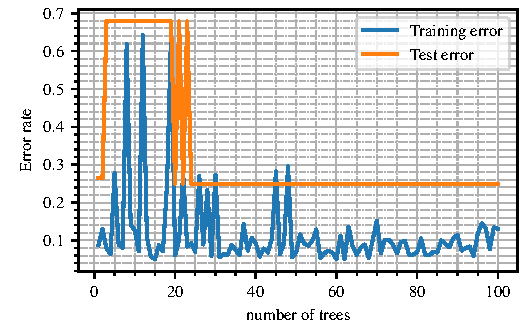
\includegraphics[scale=1.0,trim={0cm 0cm 0cm 0cm},clip]{./code/generatedPlots/q2i_error_rate.pdf}
	\caption{Q2.i: Random Forest with $m=3$: Training and test error decreases as number of trees increases}
	\label{fig:q2i_error_rate}
\end{figure}
%----------------------------------------------------------------------------------------
%	SOLUTION 2.ii
%----------------------------------------------------------------------------------------
\subsection*{Solution 2.ii}
\paragraph{Summary:} In this part we are required to plot the training and test error as we increase $m$, the number of randomly selected features to use for classification for each stump in the forest. 
\paragraph{Results:} Fig.~\ref{fig:q2ii_error_rate} shows the plot of training and test error as we increase $m$. It can be seen that both training and test error decrease with increase in $m$, however, when $m$ approaches $d$, total number of features, the error sometimes increases due to increased variance of the tree output. As, we bootstrap the training sample set before learning, each tree is trained on different sample sets which produces poor generalization accuracy if $m$ is equal to $d$. 
%%%%%%%%%%%%%%%%%%%%%%% RF ERROR VS. M %%%%%%%%%%%%%%%%%%%%%
\begin{figure}[!h]
	\centering
	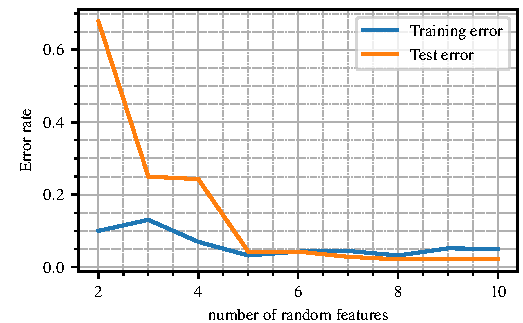
\includegraphics[scale=1.0,trim={0cm 0cm 0cm 0cm},clip]{./code/generatedPlots/q2ii_error_rate.pdf}
	\caption{Q2.ii: Random Forest with varying $m$: Training and test error}
	\label{fig:q2ii_error_rate}
\end{figure}
Fig.~\ref{fig:q2ii_error_rate_trn} shows the training error rates for different values of $m$ as we increase the number of trees. It can be seen that increasing $m$, in general decreases the error rate of random forest algorithm. The figure reveals that for any particular number of trees, increasing $m$ decreases the training error. 
%%%%%%%%%%%%%%%%%%%%%%% RF ERROR VS. M %%%%%%%%%%%%%%%%%%%%%
\begin{figure}[!h]
	\centering
	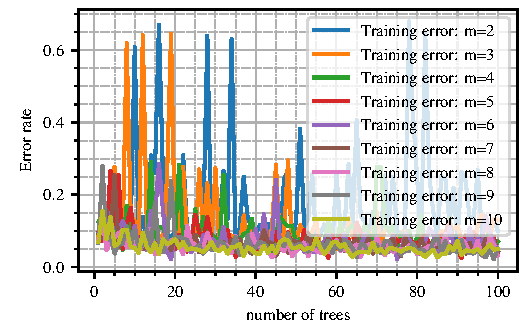
\includegraphics[scale=1.0,trim={0cm 0cm 0cm 0cm},clip]{./code/generatedPlots/q2ii_error_rate_trn.pdf}
	\caption{Q2.ii: Random Forest with varying $m$: Training error}
	\label{fig:q2ii_error_rate_trn}
\end{figure}
Fig.~\ref{fig:q2ii_error_rate_tst} shows the test error rates for different values of $m$ as we increase the number of trees. Similar trend, as we have seen in case of training error, can be seen for test error also.
%%%%%%%%%%%%%%%%%%%%%%% RF ERROR VS. M %%%%%%%%%%%%%%%%%%%%%
\begin{figure}[!h]
	\centering
	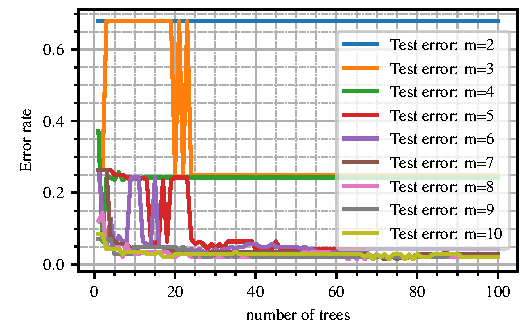
\includegraphics[scale=1.0,trim={0cm 0cm 0cm 0cm},clip]{./code/generatedPlots/q2ii_error_rate_tst.pdf}
	\caption{Q2.ii: Random Forest with varying $m$: Test error}
	\label{fig:q2ii_error_rate_tst}
\end{figure}
    %----------------------------------------------------------------------------------------
%	SOLUTION 3.a
%----------------------------------------------------------------------------------------
\subsection*{Solution 3.a}
\paragraph{Summary:} Here Tensorflow is used to build a convolutional neural network as asked in the homework. The network is learned using stochastic gradient descent (SGD) as the optimizer to update the weights without momentum and with a learning rate of $0.01$. The parameters are tuned after iterating through multiple runs with different learning rates. The value which produced best accuracy is used. I have used batch normalization layer after convolution layer to normalize the output of the convolution layer. Batch normalization is actually standardization procedure over mini batches where the convolved ensemble feature mean is subtracted from each feature and divided by the standard deviation of corresponding feature. It helps in improving the accuracy. Once the output is normalized, I have used the ReLU activation layer. Another alternative to this could be to directly pass the \textit{activation='relu'} argument to convolution layer in Tensorflow Keras.

For SGD, I have used learning rate of $0.01$ with no momentum. For ADAGRAD, I have used learning rate of $0.1$ with initial accumulator value of $0.01$. For ADAM, I have used learning rate of $0.001$ and $\rho_1$ and $\rho_2$ values of $0.9$ and $0.999$ respectively. I ran the code multiple times with different set of hyperparameters and the chose the values which produced best accuracy. For ADAM, it seemed to me that the default values gave me the best result. I have also converted labels to \textit{one-hot} representation to use \textit{categorical crossentropy} as the loss for Tensorflow model. The input features are scaled to $[0, 1]$ as I have seen this improves the performance of the neural network a lot.
\paragraph{Convergence criteria used:} I have declared convergence if in $3$ consecutive epochs the decrease of loss is less than $0.001$ or loss increases for $3$ consecutive epochs. The maximum number of epochs has a limit of $100$ though I have never seen hitting this limit before convergence is achieved.
%----------------------------------------------------------------------------------------
%	SOLUTION 3.a
%----------------------------------------------------------------------------------------
\paragraph{Results:} Fig.~\ref{fig:q3_sgd_loss_acc} shows the cumulative loss and accuracy with increasing nuber of epochs.
%%%%%%%%%%%%%%%%%%%%%%% SGD LOSS + ACCURACY %%%%%%%%%%%%%%%%%%%%%
\begin{figure}[!h]
	\centering
	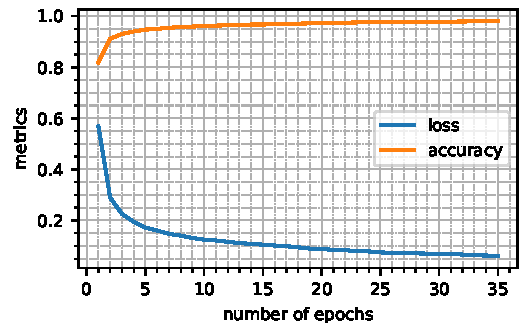
\includegraphics[scale=1.0,trim={0cm 0cm 0cm 0cm},clip]{./code/generatedPlots/q3_sgd_loss_acc.pdf}
	\caption{Q3: SGD cumulative training loss and accuracy with different epochs: CNN}
	\label{fig:q3_sgd_loss_acc}
\end{figure}
From Fig.~\ref{fig:q3_sgd_loss_acc}, we can see that as we increase the number of epochs, the network learns better and thus the loss decreases monotonically and the accuracy increases. Table~\ref{tbl:q3_sgd_loss_acc} shows the training loss and accuracy after convergence and test loss and accuracy.
%%%%%%%%%%%%%%%%%%%%%%%%%% TRAIN+TEST %%%%%%%%%%%%%%%%%%%%%%%%%%%%%%%%%%%
\begin{table}[ht]
	\centering
	\caption{Q3: Train (after convergence) and test loss and accuracy}
	\begin{tabular}[t]{ccc} 
		\hline
		& Loss & Accuracy(\%)\\ [0.5ex] 
		\hline
		Train 	& $0.060$ 	& $98.04$\\
		Test 	& $0.032$ 	& $98.93$\\[1ex]
		\hline
	\end{tabular}
	\label{tbl:q3_sgd_loss_acc}
\end{table}
If we compare the results shown in Table~\ref{tbl:q2_sgd_loss_acc} with that of Table~\ref{tbl:q3_sgd_loss_acc}, we can see that though feed forward network gave a slightly better accuracy for training data, CNN gave better test accuracy.
%----------------------------------------------------------------------------------------
%	SOLUTION 3.b
%----------------------------------------------------------------------------------------
\subsection*{Solution 3.b}
\paragraph{Convergence time calculation:} I have calculated the convergence time in seconds using the Tensorflow callbacks which is essentially the time between the train end and train begin callbacks. I have measured the time using \textit{time.time()} module of Python. Also, I have averaged the time over $10$ independent runs to reduce the variability.
\paragraph{Results:} Fig.~\ref{fig:q3_sgd_conv_time}, Fig.~\ref{fig:q3_adagrad_conv_time} and Fig.~\ref{fig:q3_adam_conv_time} show the evolution of convergence time, averaged over $10$ runs, with increasing batch size. 
%%%%%%%%%%%%%%%%%%%%%%% CONVERGENCE TIME %%%%%%%%%%%%%%%%%%%%%
\begin{figure}[!h]
	\centering
	\subfloat[][SGD: Convergence time, averaged over 10 runs, with increasing batch size]{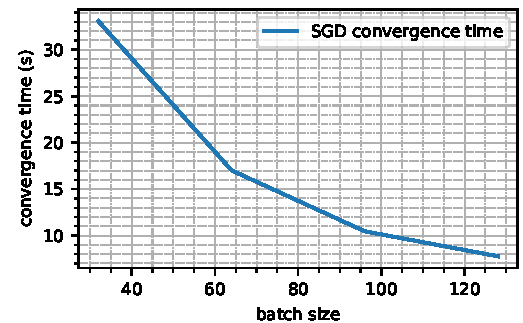
\includegraphics[scale=0.97,trim={0cm 0cm 0cm 0cm},clip]{./code/colabPlots/q3_sgd_conv_time.pdf}\label{fig:q3_sgd_conv_time}}\hspace{0.5cm}
	\subfloat[][ADAGRAD: Convergence time, averaged over 10 runs, with increasing batch size]{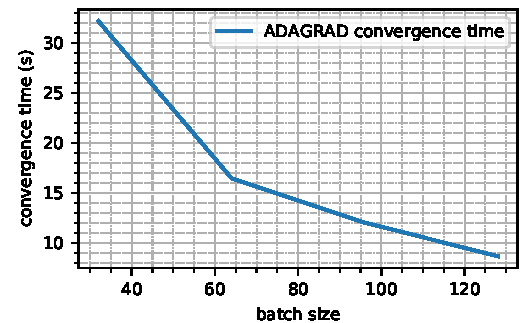
\includegraphics[scale=0.97,trim={0.0cm 0cm 0cm 0cm},clip]{./code/colabPlots/q3_adagrad_conv_time.pdf}\label{fig:q3_adagrad_conv_time}}\hspace{0.5cm}
	\subfloat[][ADAM: Convergence time, averaged over 10 runs, with increasing batch size]{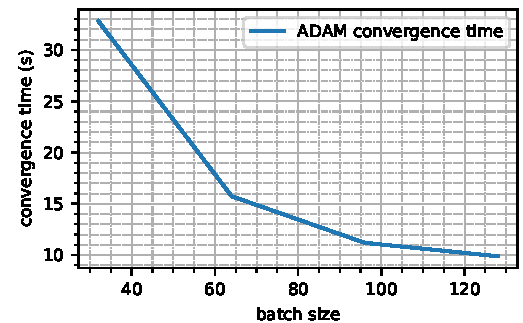
\includegraphics[scale=0.97,trim={0.0cm 0cm 0cm 0cm},clip]{./code/colabPlots/q3_adam_conv_time.pdf}\label{fig:q3_adam_conv_time}}
	\caption{Q3: CNN: Convergence time, averaged over 10 runs, with SGD, ADAGRAD and ADAM optimizer with increasing batch size}
	\label{fig:q3_conv_time}
\end{figure}
%%%%%%%%%%%%%%%%%%%%%%% CONVERGENCE TIME ALL %%%%%%%%%%%%%%%%%%%%%
\begin{figure}[!h]
	\centering
	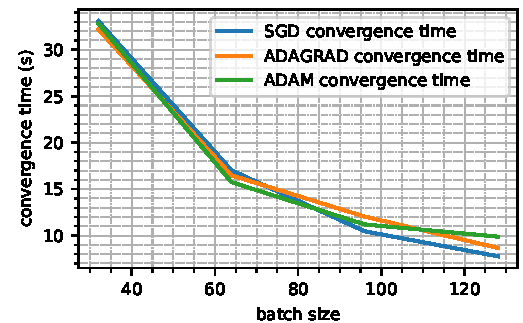
\includegraphics[scale=1.0,trim={0cm 0cm 0cm 0cm},clip]{./code/colabPlots/q3_all_conv_time.pdf}
	\caption{Q3: CNN: Convergence time comparison, averaged over 10 runs, with SGD, ADAGRAD and ADAM optimizer with increasing batch size}
	\label{fig:q3_all_conv_time}
\end{figure}


From Fig.~\ref{fig:q3_sgd_conv_time}, Fig.~\ref{fig:q3_adagrad_conv_time}, Fig.~\ref{fig:q3_adam_conv_time} and Fig.~\ref{fig:q3_all_conv_time}, we can see that as we increase the batch size the time taken to converge in seconds decreases which means learning becomes faster as we increase the batch size. However, this is opposite to the theoretical understanding we have on the effect of increasing batch size as we know if we increase the number of batch size, gradient computation time increases and thus learning time becomes slower. Thus, I believe, in this case, the CPU instructions or parallelization is playing a major role in deciding the convergence time. I have used \textit{time.time()} module of Python to compute the convergence time. I have also tested the code on Google Colab with GPU. Both CPU and GPU generated same trend of decreasing convergence time with increasing batch size. Therefore, I believe, here the convergence time (in seconds) is primarily governed by how the code execution is being handled by the CPU or GPU. I cross checked it with Professor and we agreed that it could be a possible reason of seeing this trend. Another possibility could be to plot iteration number instead of time in seconds on y-axis, however, we agreed to exclude that detail for this homework.
\newpage
\paragraph{Details gathered from a single run:} Fig.~\ref{fig:q3_loss_acc_32} shows the loss and accuracy for SGD, ADAGRAD and ADAM optimizers for a single run with batch size of $32$. The figures reveal that of all these three optimizers, ADAM performs best.
%%%%%%%%%%%%%%%%%%%%%%% CONVERGENCE TIME %%%%%%%%%%%%%%%%%%%%%
\begin{figure}[!h]
	\centering
	\subfloat[][Q3: CNN: Accuracy of different optimizer with 32 batch size]{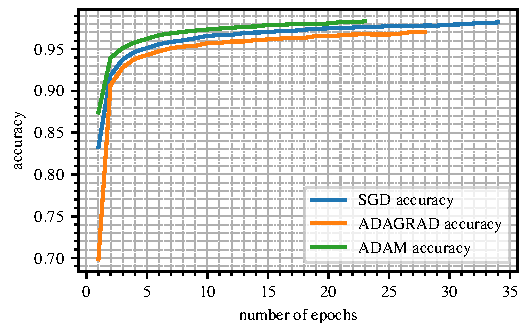
\includegraphics[scale=0.97,trim={0.0cm 0cm 0cm 0cm},clip]{./code/generatedPlots/q3_acc_batch_32.pdf}\label{fig:q3_acc_batch_32}}\hspace{0.5cm}
	\subfloat[][Q3: CNN: loss of different optimizer with 32 batch size]{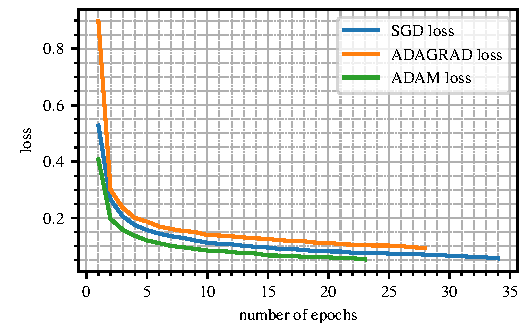
\includegraphics[scale=0.97,trim={0.0cm 0cm 0cm 0cm},clip]{./code/generatedPlots/q3_loss_batch_32.pdf}\label{fig:q3_loss_batch_32}}\hspace{0.5cm}
	\caption{Q3: CNN: Accuracy and loss with SGD, ADAGRAD and ADAM optimizer with increasing epoch with batch size of 32}
	\label{fig:q3_loss_acc_32}
\end{figure}
Fig.~\ref{fig:q3_loss_acc_64} shows the loss and accuracy for SGD, ADAGRAD and ADAM optimizers for a single run with batch size of $64$. The figures reveal that of all these three optimizers, ADAM performs best.
%%%%%%%%%%%%%%%%%%%%%%% CONVERGENCE TIME %%%%%%%%%%%%%%%%%%%%%
\begin{figure}[!h]
	\centering
	\subfloat[][Q3: CNN: Accuracy of different optimizer with 64 batch size]{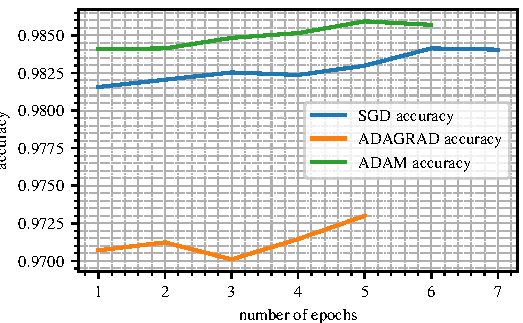
\includegraphics[scale=0.97,trim={0.0cm 0cm 0cm 0cm},clip]{./code/generatedPlots/q3_acc_batch_64.pdf}\label{fig:q3_acc_batch_64}}\hspace{0.5cm}
	\subfloat[][Q3: CNN: loss of different optimizer with 64 batch size]{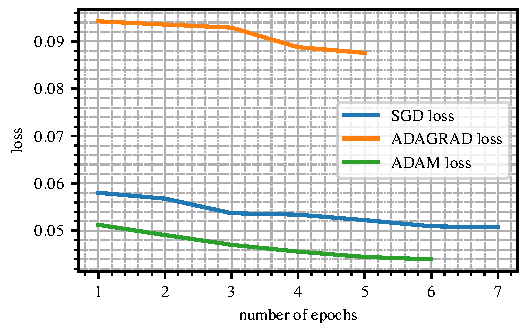
\includegraphics[scale=0.97,trim={0.0cm 0cm 0cm 0cm},clip]{./code/generatedPlots/q3_loss_batch_64.pdf}\label{fig:q3_loss_batch_64}}\hspace{0.5cm}
	\caption{Q3: CNN: Accuracy and loss with SGD, ADAGRAD and ADAM optimizer with increasing epoch with batch size of 64}
	\label{fig:q3_loss_acc_64}
\end{figure}
Fig.~\ref{fig:q3_loss_acc_96} shows the loss and accuracy for SGD, ADAGRAD and ADAM optimizers for a single run with batch size of $96$. The figures reveal that of all these three optimizers, ADAM performs best.
%%%%%%%%%%%%%%%%%%%%%%% CONVERGENCE TIME %%%%%%%%%%%%%%%%%%%%%
\begin{figure}[!h]
	\centering
	\subfloat[][Q3: CNN: Accuracy of different optimizer with 96 batch size]{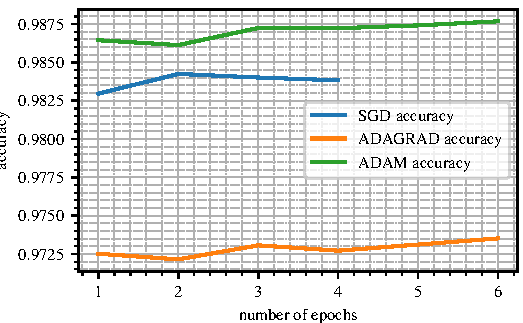
\includegraphics[scale=0.97,trim={0.0cm 0cm 0cm 0cm},clip]{./code/generatedPlots/q3_acc_batch_96.pdf}\label{fig:q3_acc_batch_96}}\hspace{0.5cm}
	\subfloat[][Q3: CNN: loss of different optimizer with 96 batch size]{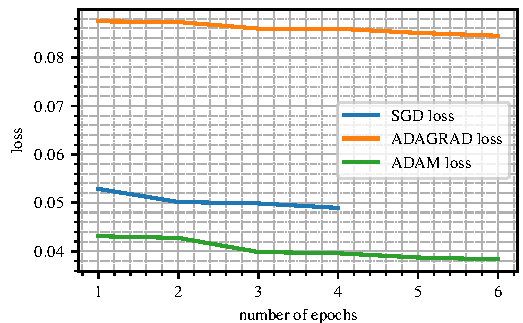
\includegraphics[scale=0.97,trim={0.0cm 0cm 0cm 0cm},clip]{./code/generatedPlots/q3_loss_batch_96.pdf}\label{fig:q3_loss_batch_96}}\hspace{0.5cm}
	\caption{Q3: CNN: Accuracy and loss with SGD, ADAGRAD and ADAM optimizer with increasing epoch with batch size of 96}
	\label{fig:q3_loss_acc_96}
\end{figure}
Fig.~\ref{fig:q3_loss_acc_128} shows the loss and accuracy for SGD, ADAGRAD and ADAM optimizers for a single run with batch size of $128$. The figures reveal that of all these three optimizers, ADAM performs best.
%%%%%%%%%%%%%%%%%%%%%%% CONVERGENCE TIME %%%%%%%%%%%%%%%%%%%%%
\begin{figure}[!h]
	\centering
	\subfloat[][Q3: CNN: Accuracy of different optimizer with 128 batch size]{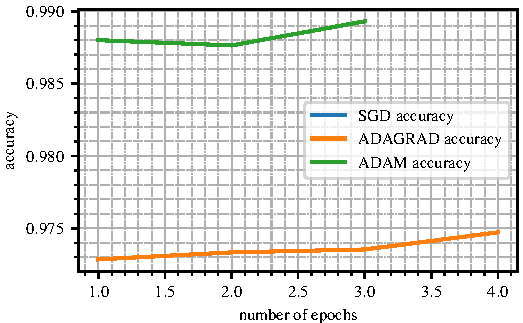
\includegraphics[scale=0.97,trim={0.0cm 0cm 0cm 0cm},clip]{./code/generatedPlots/q3_acc_batch_128.pdf}\label{fig:q3_acc_batch_128}}\hspace{0.5cm}
	\subfloat[][Q3: CNN: loss of different optimizer with 128 batch size]{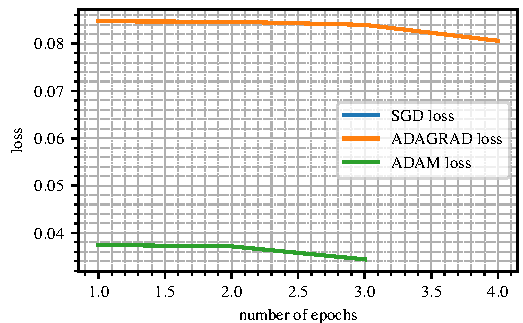
\includegraphics[scale=0.97,trim={0.0cm 0cm 0cm 0cm},clip]{./code/generatedPlots/q3_loss_batch_128.pdf}\label{fig:q3_loss_batch_128}}\hspace{0.5cm}
	\caption{Q3: CNN: Accuracy and loss with SGD, ADAGRAD and ADAM optimizer with increasing epoch with batch size of 128}
	\label{fig:q3_loss_acc_128}
\end{figure}
    %%----------------------------------------------------------------------------------------
%	SOLUTION 4
%----------------------------------------------------------------------------------------
\subsection*{Solution 4}
\paragraph{Logistic regression (LR):} Let $N, K, x\in \mathbb{R}^d, C_i, w_i \in \mathbb{R}^d, w_{i0} \in \mathbb{R}$ denote number of samples, number of classes, data sample, $i^{th}$ class, weights and intercept of the linear model respectively. For logistic regression, I use the $softmax$ function, as shown below, to find the posterior:
\begin{align*}
y_i = \hat{P}(C_i | x) = \frac{\text{exp}[w_i^Tx + w_{i0}]}{\sum_{j=1}^K\text{exp}[w_j^Tx + w_{j0}]},
\end{align*}
for all $i \in \{1,2,\ldots, K\}$. The error function is
\begin{align*}
E = -\sum_{t=1}^N \sum_{i=1}^K r_i^t \log(y_i),
\end{align*}
where $r_i^t = 1$ if $x^t \in C_i$ and $0$ otherwise. The objective is to find optimal values of $w_i, w_{i0}$ for all $i \in \{1,2,\ldots,K\}$ such that the error $E$ is minimized. I use gradient descent to find the updates to $w_i, w_{i0}$. The gradient of $E$ with respect to $w_i$ is
\begin{align*}
\frac{\partial E}{\partial w_i} &= \frac{\partial E}{\partial y_i} \frac{\partial y_i}{\partial w_i}\\
&= -\sum_{t=1}^N(r_i^t - y_i^t)x^t,
\end{align*}
and
\begin{align*}
\frac{\partial E}{\partial w_{i0}} &= \frac{\partial E}{\partial y_i}\frac{\partial y_i}{\partial w_{i0}}\\
&= -\sum_{t=1}^N(r_i^t - y_i^t).
\end{align*}
Therefore, the update equation for gradient descent algorithm is
\begin{align*}
w_i^{new} &= w_i^{old} + \eta \sum_{t=1}^N(r_i^t - y_i^t)x^t,\\
w_{i0}^{new} &= w_{i0}^{old} + \eta \sum_{t=1}^N(r_i^t - y_i^t),
\end{align*}
where $\eta$ is the learning rate. I have taken $\eta=0.001$. I have also kept a provision to add regularization term in my code for which the update equation becomes,
\begin{align*}
w_i^{new} &= w_i^{old} + \eta \sum_{t=1}^N(r_i^t - y_i^t)x^t -\eta C w_i^{old},\\
w_{i0}^{new} &= w_{i0}^{old} + \eta \sum_{t=1}^N(r_i^t - y_i^t) - \eta C w_{i0}^{old},
\end{align*}
where $C$ is the regularization term which I have taken as $10$ in my code. I have used batch gradient descent.
\paragraph{Naive Bayes with marginal Gaussian distributions (GNB):} In case of Naive Bayes, we assume that the features in the samples are uncorrelated. Therefore, the covariance matrices are diagonal. The approach is similar to as described in Solution 3.ii. But to compare GNB to linear LR, we need to make use of shared covariance matrix for all classes. Therefore, we can use pooling of data to find a shared covariance matrix as follows
\begin{align}
	S = \sum_{i=1}^K \hat{P}(C_i)S_i,
\end{align}
where $\hat{P}(C_i), S_i$ are defined in~(\ref{eq:mle}). Now, if we use $S$ in place of $S_i$ for all $i \in \{1,2,\ldots,K\}$ in~(\ref{eq:disc_func}), we can see that the term $-\frac{1}{2}\log(|S|)$ becomes common to all discriminators. Therefore, we can drop this term and use
\begin{align*}
	g_i(x) = -\frac{1}{2}(x-m_i)^TS^{-1}(x-m_i) + \log(\hat{P}(C_i)).
\end{align*}
as the discriminator. In this case, we see that the quadratic term $\frac{1}{2}x^TS^{-1}x$ becomes common to all discriminators, thus, the discriminator gives rise to a linear function of $x$ which can be compared to LR model.
\paragraph{Results:} Fig.~\ref{fig:boston50_test_err}, Fig.~\ref{fig:boston75_test_err} and Fig.~\ref{fig:digits_test_err} show the test data error percentage for LR anf GNB model, for `Boston50', `Boston75' and `Digits' data respectively, with percentage of training data used to train the model in x-axis. It can be seen that the LR model performs better than GNB.
\begin{figure}[h]
	\centering
	\subfloat[][Test set error plot on Boston50 dataset]{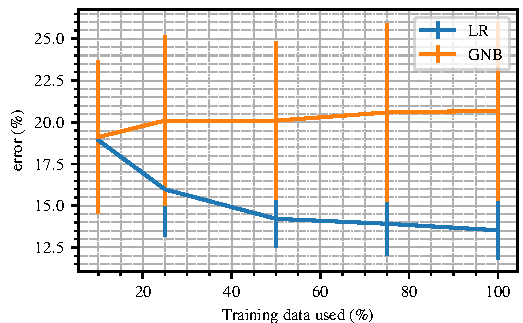
\includegraphics[scale=1.0,trim={0cm 0cm 0cm 0cm},clip]{./code/generatedPlots/Q4_boston50_test_err.pdf}
	\label{fig:boston50_test_err}}\hspace*{0.5cm}
	\subfloat[][Test set error plot on Boston75 dataset]{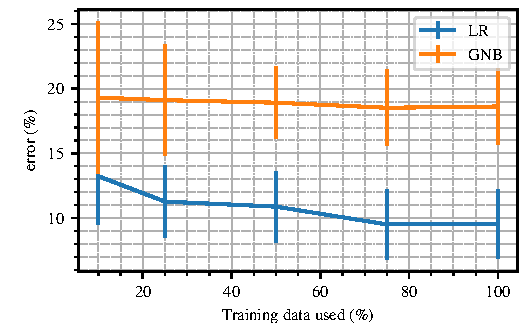
\includegraphics[scale=1.0,trim={0cm 0cm 0cm 0cm},clip]{./code/generatedPlots/Q4_boston75_test_err.pdf}
	\label{fig:boston75_test_err}}\\
	\subfloat[][Test set error plot on digits dataset]{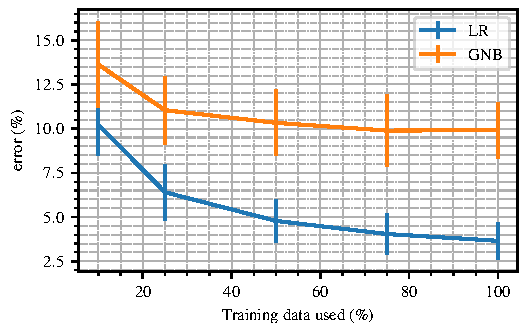
\includegraphics[scale=1.0,trim={0cm 0cm 0cm 0cm},clip]{./code/generatedPlots/Q4_digits_test_err.pdf}
	\label{fig:digits_test_err}}
	\caption{Q4: Test data error comparison between LR and GNB}
\end{figure}

    %%----------------------------------------------------------------------------------------
%	SOLUTION 5
%----------------------------------------------------------------------------------------
\subsection*{Solution 5}
The probability density function $p(x;\mu,\Sigma), x\in \mathbb{R}^d$ of a multivariate Gaussian distribution with mean $\mu \in \mathbb{R}^d$ and covariance $\Sigma \in \mathbb{R}^{d\times d}$ is
\begin{align*}
	p(x;\mu,\Sigma) = \frac{1}{(2\pi)^{\frac{d}{2}} |\Sigma|^{\frac{1}{2}}}e^{-\frac{1}{2}(x-\mu)^T\Sigma^{-1}(x-\mu)},
\end{align*}
where $|\Sigma|$ denotes the determinant of $\Sigma$.

If the precision matrix is denoted by $\Theta = \Sigma^{-1}$, then
\begin{align*}
	p(x;\mu,\Theta^{-1}) = \frac{1}{(2\pi)^{\frac{d}{2}}}|\Theta|^{\frac{1}{2}}e^{-\frac{1}{2}(x-\mu)^T\Theta(x-\mu)},
\end{align*}
where $|\Theta|$ is the determinant of the precision matrix $\Theta$.

    %\input{problem_2}
    %\input{solution_2}
\end{document}